\section{L-system grammars}

According to Prusinkiewicz and Hanan a simple type of L-systems are those known as deterministic 0L systems, where the string refers to the sequence of cellular states and '0L system' abbreviating 'Lindenmayer system with zero-sided interactions'.  With 0L systems there are only three major parts. There is a set of symbols (\textit{alphabet}), the starting string (\textit{Axiom}) and state transition rules (\textit{rules}). The alphabet is a set of states. The starting string is a starting point containing one or more states. The transition rules are rules that dictate whether a state should remain the same or transition into a different state or even disappear. \cite{prusinkiewicz2013lindenmayer}. \\
\\
An example of a deterministic 0L system is that a simplified model for the growth of algae: \\
\\
We are given the \textit{alphabet}: A, B \\ 
and the \textit{axiom}: A \\
and the \textit{rule} set: \\ 
A $\rightarrow$ AB \\
B $\rightarrow$ A \\
\\
If we then apply the rules to the L-system we find it creates the following generation structure. \\
1.) A \\
2.) AB \\
3.) ABA \\
4.) ABAAB \\
5.) ABAABABA \\
6.) ABAABABAABAAB \\
\\
This rewriting of initial string using a set of rules is ultimately the underlying concept behind L-systems. There are a number of improvements that can be made to this type of L-system in order to accommodate for more complex and intricate structure. One of which is the inclusion of \textit{constants}. Constants can be considered any state that does not have a rule associated with it or remains the same from generation to generation and therefore holds a consistent value or meaning. Some examples of constants are stated below. \\
\\
$\bullet$ +: Rotate to the right specified angle. \\
$\bullet$ -: Rotate to the left by a specified angle.  \\
$\bullet$ [: Save the current position and angle. \\
$\bullet$ ]: Load a saved position and angle. \\
\\
These types of constants are useful when we are dealing with fractal structures.

\section{Basic 2D L-systems} 

There are a number of fractal geometry that have become well known particularly with regards to how they can seemingly imitate nature \cite{mandelbrot1982fractal}. Particularly with the geometry such as the Koch snowflake which can be represented using the following L-system.

\begin{figure}[htbp]
	\raggedright
	\textbf{\underline{Koch Curve:}} \\
	\textbf{Alphabet:} F \\
	\textbf{Constants:} +, - \\
	\textbf{Axiom:} F \\
	\textbf{Angle:} 90$^\circ$ \\
	\textbf{Rules:} \\
	F $\rightarrow$ F+F--F+F\\
	{\centering
		\vspace{7px}
		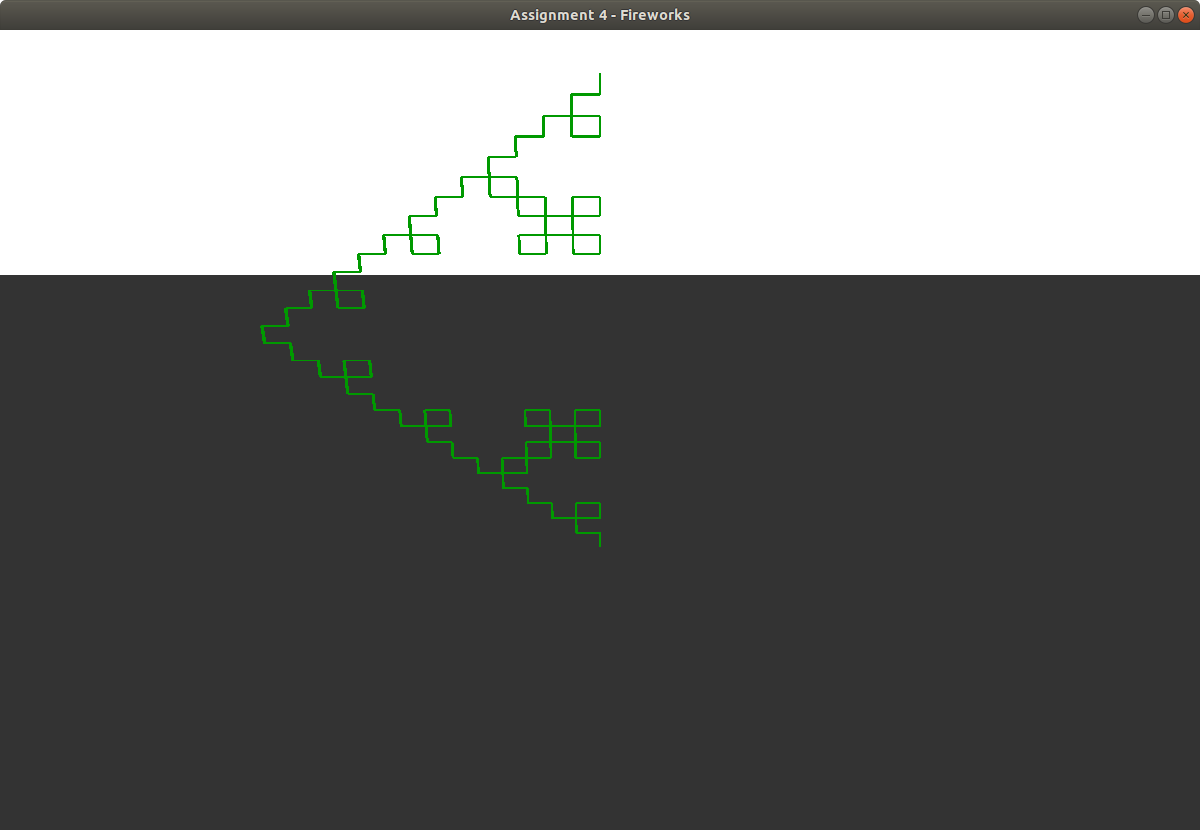
\includegraphics[scale=0.8]{KochCurve/KochCurve04.png}
		\caption{Koch Curve.}
	}
\end{figure}
\begin{figure}[htbp]
	\raggedright
	\textbf{\underline{Sierpinski Triangle:}} \\
	\textbf{Alphabet:} A, B \\
	\textbf{Constants:} +, - \\
	\textbf{Axiom:} A \\
	\textbf{Angle:} 60$^\circ$ \\
	\textbf{Rules:} \\
	A $\rightarrow$  B-A-B \\
	B $\rightarrow$ A+B+A\\
	{\centering
		\vspace{7px}
		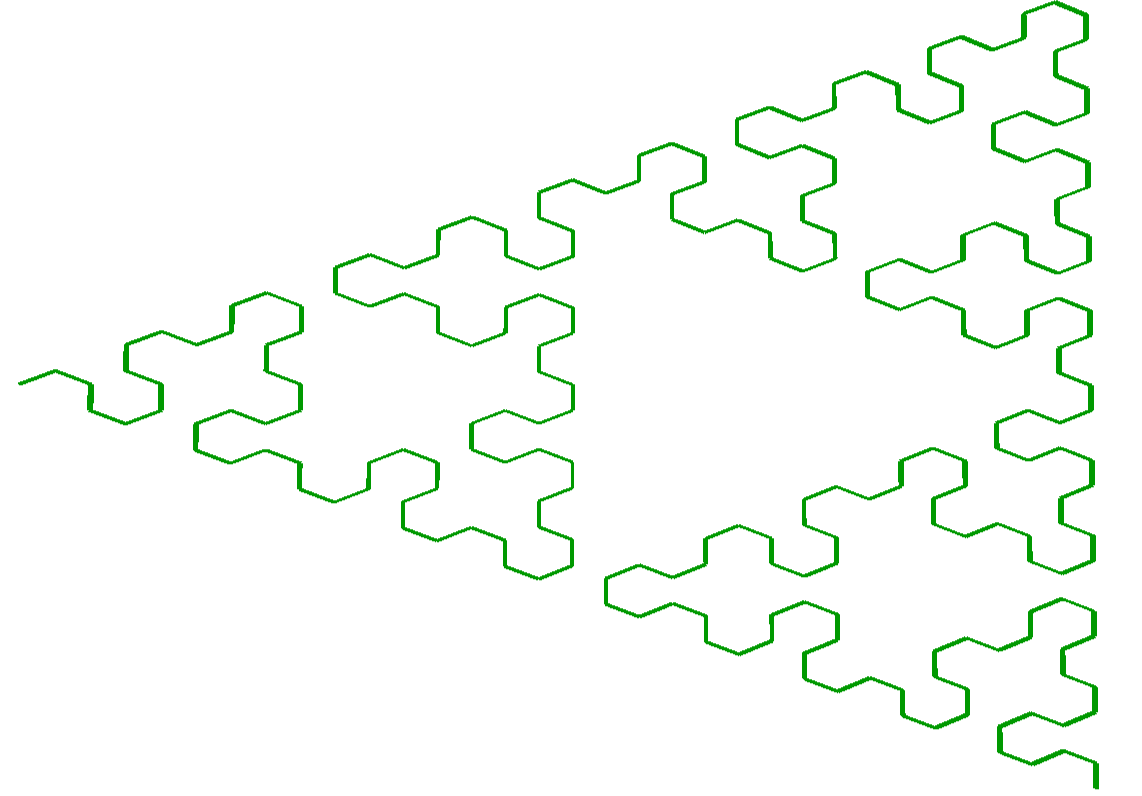
\includegraphics[scale=0.17]{SierpinskiTriangle/SierpinskiTriangle06.png}
		\caption{Sierpinski Triangle.}
	}
\end{figure}
\begin{figure}[htbp]
	\raggedright
	\textbf{\underline{Dragon Curve:}} \\
	\textbf{Alphabet:} F, X, Y \\
	\textbf{Constants:} +, - \\
	\textbf{Axiom:} FX \\
	\textbf{Angle:} 90$^\circ$ \\
	\textbf{Rules:} \\
	X $\rightarrow$ X+YF+ \\
	Y $\rightarrow$ -FX-Y\\
	{\centering
		\vspace{7px}
		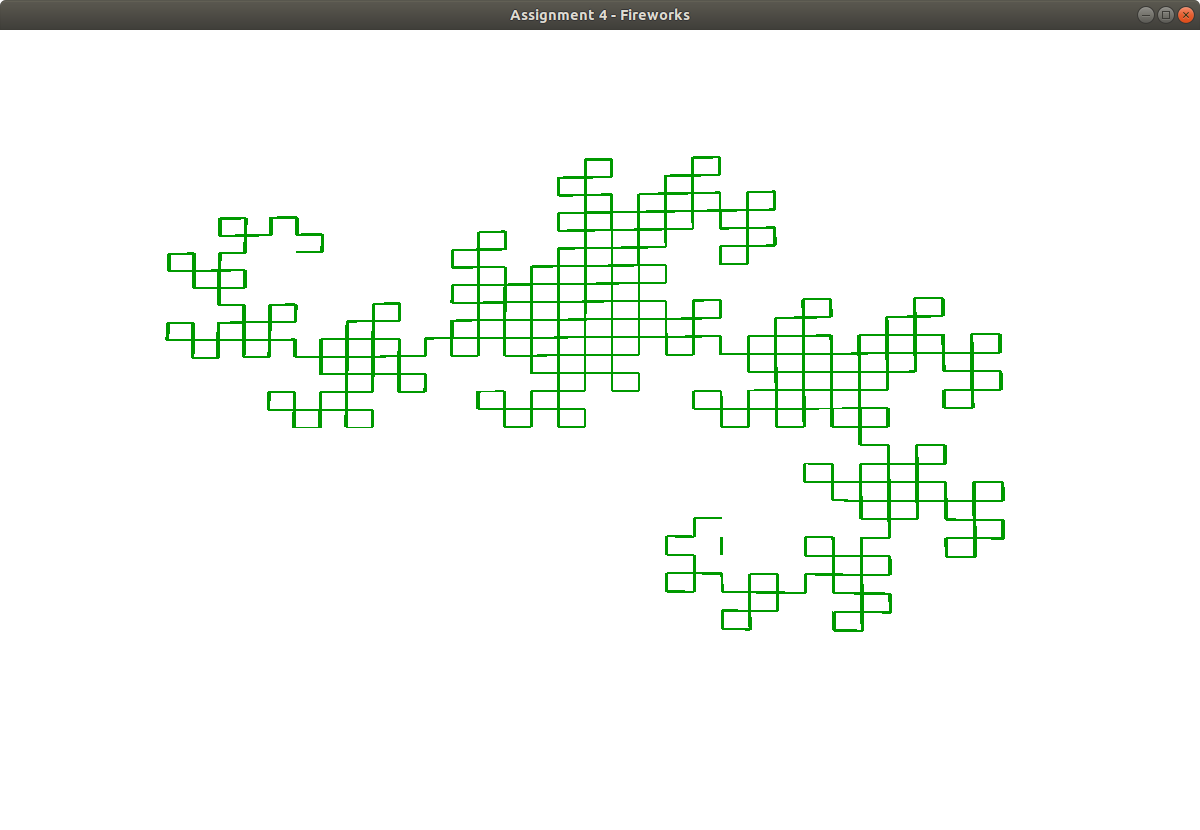
\includegraphics[scale=0.17]{DragonCurve/DragonCurve10.png}
		\caption{Dragon Curve.}
	}
\end{figure}
\begin{figure}[htbp]
	\raggedright
	\textbf{\underline{Fractal Plant:}} \\
	\textbf{Alphabet:} X, F\\
	\textbf{Constants:} +, -, [, ] \\
	\textbf{Axiom:} X \\
	\textbf{Angle:} 25$^\circ$ \\
	\textbf{Rules:} \\
	X $\rightarrow$ F-[[X]+X]+F[+FX]-X\\
	F $\rightarrow$ FF \\
	{\centering
		\vspace{7px}
		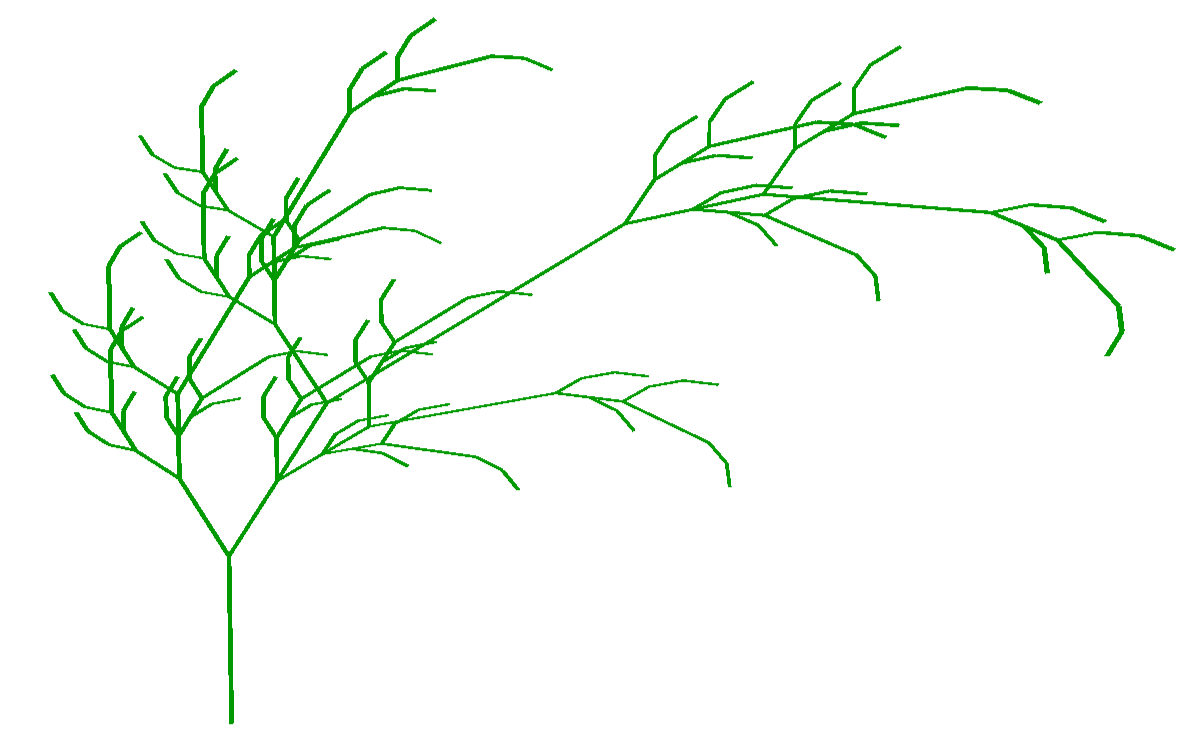
\includegraphics[scale=0.15]{FractalPlant/FractalPlant05.png}
		\caption{Fractal Plant.}
	}
\end{figure}
\begin{figure}[htbp]
	\raggedright
	\textbf{\underline{Fractal Bush:}} \\
	\textbf{Alphabet:} F\\
	\textbf{Constants:} +, -, [, ] \\
	\textbf{Axiom:} F \\
	\textbf{Angle:} 25$^\circ$ \\
	\textbf{Rules:} \\
	F $\rightarrow$ FF+[+F-F-F]-[-F+F+F]\\
	{\centering
		\vspace{7px}
		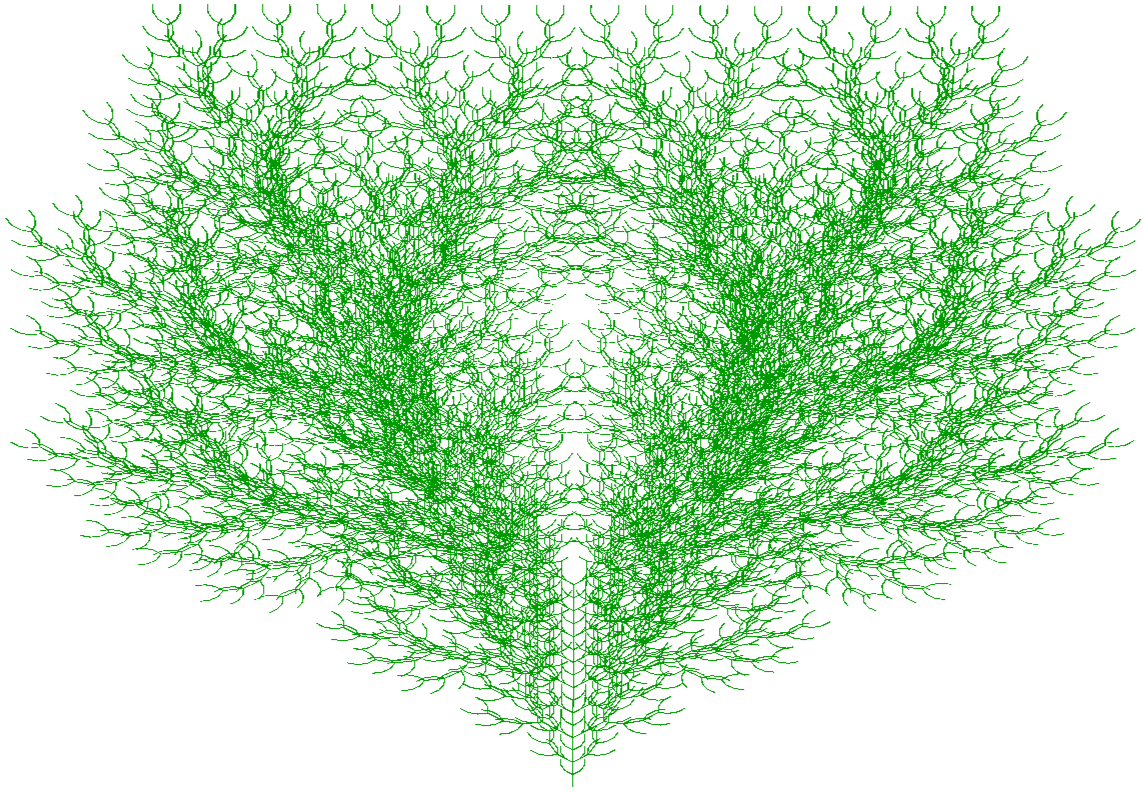
\includegraphics[scale=0.15]{FractalBush/FractalBush06.png}
		\caption{Fractal Bush.}
	}
\end{figure}

\FloatBarrier
\newpage
\section{Branching Filaments}